\section{Computational study}
\label{sec:exp}

\subsection{Design and protocol}
We evaluate selection \emph{quality} under a held-out protocol: each method picks
one alternative using only its own machinery, and the pick is scored against
preference models that \emph{no} method used during selection. To avoid biasing
the evaluation toward the additive/scalarising logic of the probes, the held-out
set spans \textbf{six} families---random linear $-w^\top r$, weighted Chebyshev
$-\max_i w_i r_i$, augmented ASF, CES, a \emph{non-additive} $2$-additive Choquet
integral with random non-negative M\"obius masses on singletons and pairs, and a
\emph{satisficing} threshold utility penalising exceedances of random aspiration
levels. Weights are drawn from a uniform simplex; $300$ utilities are sampled per
family per replication. We report two non-negative, lower-is-better losses,
each normalised per utility against the best and worst feasible alternatives: the
\emph{mean held-out loss} and the \emph{tail held-out loss} (mean of the worst
$10\%$ of per-utility losses, a CVaR-style worst-case measure that LUR targets).

Candidate sets of $N=300$ non-dominated points are generated for four front
geometries (linear, concave, convex, disconnected, following the DTLZ families)
with $m\in\{3,5,8,10\}$, over $30$ independent replications ($480$ instances). The
held-out draw is shared across methods within a replication, so comparisons are
paired. \textbf{Baselines and parameters.} TOPSIS, compromise programming (CP,
$p{=}2$), knee selection (distance-to-hyperplane), achievement scalarisation (ASF,
reference at the ideal), and a random-weight popularity rule (RW) all use equal
weights where applicable. The robust-MCDA baselines use $1000$ Monte-Carlo
simplex weights: \textbf{SMAA} recommends the alternative with the highest
first-rank acceptability index (ties broken by expected value); \textbf{MMR}
minimises the maximum Savage regret over the same weight set. LUR uses the
adaptive probe family with $\theta=0.6$ and the tolerance-based leximax rule.
Significance is assessed by the Friedman test with Nemenyi critical difference
(CD) and by Holm-corrected Wilcoxon signed-rank tests against LUR with Cliff's
$\delta$ effect size.

\subsection{Overall results}
Table~\ref{tab:main} reports mean and tail loss averaged over all geometries and
$m$. On \emph{tail} loss the four robust/compromise methods MMR ($0.470$), ASF
($0.472$), LUR ($0.481$) and CP ($0.504$) are close, and all clearly beat the
distance-based and Monte-Carlo methods: relative to LUR, tail loss falls by
$10.8\%$ vs TOPSIS ($0.539$), $20.6\%$ vs knee ($0.606$), $46.6\%$ vs RW
($0.900$) and $47.4\%$ vs SMAA ($0.914$). Figure~\ref{fig:cd} shows the
average-rank CD diagram (Friedman $p<10^{-15}$, $n=480$, CD $=0.48$). Read
rigorously: \textbf{LUR is statistically indistinguishable from CP} (rank gap
$0.02$) and \textbf{very slightly behind the two best methods MMR and ASF} (gaps
$0.59$ and $0.50$, just beyond CD)---but the corresponding effect sizes are
\emph{negligible} (Cliff's $|\delta|\le 0.034$). Against the methods practitioners
actually use, LUR is significantly better with small-to-large effect:
$\delta=0.087$ (TOPSIS), $0.285$ (knee), $0.850$ (RW), $0.873$ (SMAA), all
$p<10^{-4}$. We therefore claim only that \emph{LUR is in the best-performing
group on worst-case loss and far better than averaging/Monte-Carlo selection}, not
that it dominates the strongest robust scalarisations. On \emph{mean} loss the
averaging methods (CP, MMR) lead and LUR is mid-pack---the expected price of
worst-case robustness (\S\ref{sec:disc}).

\begin{table}[t]
\centering\small
\caption{Held-out loss over four geometries $\times$ $m\in\{3,5,8,10\}$, 30
replications (480 instances; lower is better). Tail loss is the worst-case
(CVaR$_{10\%}$) metric. Best in each column in \textbf{bold}; on tail loss LUR is
within a negligible effect size ($|\delta|\le0.034$) of MMR/ASF/CP.}
\label{tab:main}
\begin{tabular}{lcc}
\toprule
Method & mean loss & tail loss\\
\midrule
TOPSIS & 0.220 & 0.539\\
CP     & \textbf{0.207} & 0.504\\
Knee   & 0.308 & 0.606\\
RW     & 0.462 & 0.900\\
ASF    & 0.234 & 0.472\\
SMAA   & 0.468 & 0.914\\
MMR    & 0.228 & \textbf{0.470}\\
\textbf{LUR} & 0.245 & 0.481\\
\bottomrule
\end{tabular}
\end{table}

\begin{figure}[t]
\centering
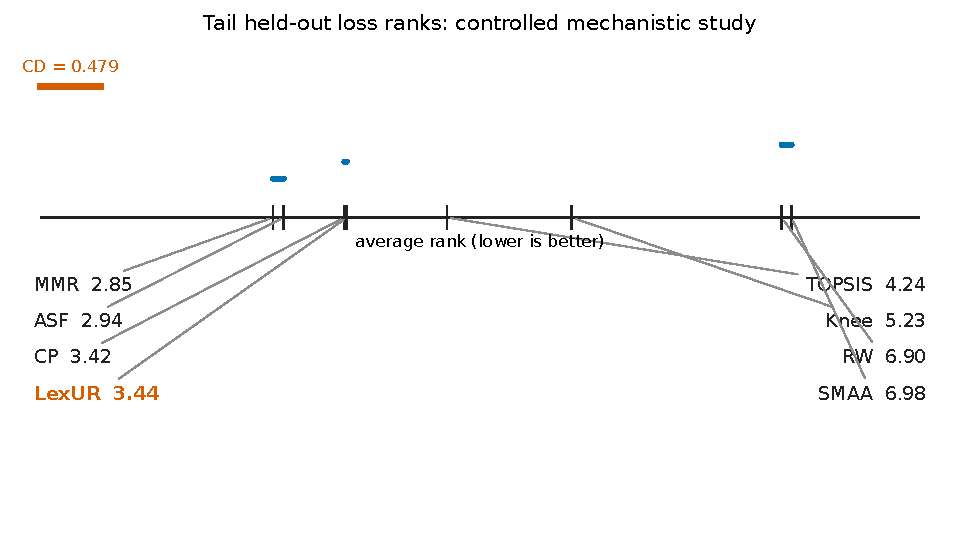
\includegraphics[width=0.85\textwidth]{cd_diagram.pdf}
\caption{Average ranks on tail (worst-case) held-out loss with Nemenyi critical
difference ($n=480$, $\alpha=0.05$, CD $=0.48$). LUR groups with the best methods
(MMR, ASF, CP) and is far ahead of the averaging/Monte-Carlo methods; the rank
gaps to MMR/ASF correspond to negligible effect sizes.}
\label{fig:cd}
\end{figure}

\subsection{Behaviour across preference families}
Table~\ref{tab:family} breaks the loss down by held-out family on a representative
setting (concave, $m=8$), including the two non-additive families. The structure
is a clear trade-off: averaging methods (TOPSIS, SMAA) are strong on linear
utilities but weak on the max-type families; ASF and MMR are the reverse---best on
Chebyshev/CES but worst on linear. LUR sits between the two camps: it removes much
of ASF's linear-utility weakness ($0.598$ vs $0.674$) while staying competitive on
the max-type \emph{and} the non-additive Choquet ($0.368$) and satisficing
($0.468$) families. We do \emph{not} claim LUR is the flattest profile---on this
setting CP is flatter and has the lowest overall mean ($0.404$)---only that LUR is
robust across additive and non-additive preferences without being tuned to any.

\begin{table}[t]
\centering\small
\caption{Held-out loss by preference family (concave, $m=8$, 30 replications),
including the non-additive Choquet and satisficing families. Lowest per column in
\textbf{bold}. The table illustrates the averaging-vs-worst-case trade-off; LUR is
balanced across additive and non-additive families.}
\label{tab:family}
\begin{tabular}{lccccccc}
\toprule
Method & linear & Cheby. & aug.\ ASF & CES & Choquet & satisfice & overall\\
\midrule
TOPSIS & \textbf{0.391} & 0.511 & 0.511 & 0.563 & 0.341 & 0.511 & 0.471\\
CP     & 0.486 & 0.458 & 0.458 & 0.440 & 0.307 & \textbf{0.278} & \textbf{0.404}\\
Knee   & 0.477 & 0.503 & 0.503 & 0.524 & 0.479 & 0.570 & 0.509\\
RW     & 0.403 & 0.519 & 0.519 & 0.569 & 0.379 & 0.552 & 0.490\\
ASF    & 0.674 & 0.434 & 0.434 & \textbf{0.329} & \textbf{0.288} & 0.388 & 0.425\\
SMAA   & 0.398 & 0.521 & 0.521 & 0.575 & 0.367 & 0.546 & 0.488\\
MMR    & 0.653 & 0.442 & 0.443 & 0.348 & 0.344 & 0.402 & 0.439\\
\textbf{LUR} & 0.598 & 0.454 & 0.454 & 0.374 & 0.368 & 0.468 & 0.453\\
\bottomrule
\end{tabular}
\end{table}

\subsection{Certificate regret and uniformity}
By construction LUR minimises the leximax of its certificate regret. Empirically
(concave, $m=8$) LUR attains worst-case certificate regret $0.708$, far below
every alternative (MMR $0.921$, CP $0.936$, ASF $0.953$, TOPSIS $0.974$), with one
of the most uniform regret profiles (sorted-disappointment std $0.219$, second to
MMR's $0.207$). This is by design---LUR optimises exactly this object---so it is a
consistency check, not an independent win; its decision value is that the
recommendation is \emph{auditable}.

\subsection{Robustness to redundant criteria}
We test the case motivating clustering: the DM's true preferences are over $c$
underlying criteria, each measured by several redundant (positively correlated)
objectives, with held-out utilities defined on the \emph{true} criteria. The
clustering recovers the redundancy groups essentially exactly.
Table~\ref{tab:redund} (four group structures $\times$ three geometries, 30
replications) shows LUR tied with ASF for best grouped loss and in the best group
on tail loss; the averaging and Monte-Carlo methods, which amplify redundant
groups, are $19$--$35\%$ worse on grouped loss (TOPSIS $0.332$, SMAA $0.413$ vs
LUR $0.268$). As discussed in \S\ref{sec:probes}, this reflects \emph{reduced},
not eliminated, redundancy sensitivity.

\begin{table}[t]
\centering\small
\caption{Redundant-objective benchmark (true preferences over the underlying
criteria; 4 group structures $\times$ 3 geometries, 30 replications). Grouped loss
measures de-redundification quality. Lower is better; best in \textbf{bold}.}
\label{tab:redund}
\begin{tabular}{lcc}
\toprule
Method & grouped loss & tail loss\\
\midrule
TOPSIS & 0.332 & 0.455\\
CP     & 0.317 & 0.423\\
Knee   & 0.322 & 0.489\\
RW     & 0.409 & 0.598\\
ASF    & \textbf{0.266} & 0.406\\
SMAA   & 0.413 & 0.603\\
MMR    & 0.295 & \textbf{0.387}\\
\textbf{LUR} & 0.268 & 0.391\\
\bottomrule
\end{tabular}
\end{table}

\subsection{Distinctness, dominated exclusion, ablation, sensitivity}
LUR and the SMAA recommender coincide on only $1.2\%$ of instances and select
alternatives a mean normalised distance $0.86$ apart: LUR is operationally a
different rule, not a re-description of acceptability analysis. Across 200
randomised trials with injected dominated points LUR never selected a dominated
alternative ($0/200$), confirming Corollary~\ref{cor:dom}. Ablation (concave,
$m=8$): dropping the singletons raises loss ($0.456\!\to\!0.483$) and worst-case
certificate regret ($0.701\!\to\!0.783$); a max-only family lowers mean loss to
$0.420$ but inflates certificate regret to $0.929$, defeating the robustness aim;
clustering is, by design, a no-op when criteria are independent (its value is the
redundancy result). LUR is insensitive to the clustering threshold $\theta$ over
$[0.3,0.9]$ across \emph{all four} geometries (Figure~\ref{fig:sens}, left). Under
nadir-estimation error the held-out loss of the chosen alternative stays stable
($\approx0.45$ up to $50\%$ error), though the \emph{identity} of the choice
changes increasingly often (Figure~\ref{fig:sens}, right), indicating near-ties
among good alternatives rather than quality loss.

\begin{figure}[t]
\centering
\begin{subfigure}{0.48\textwidth}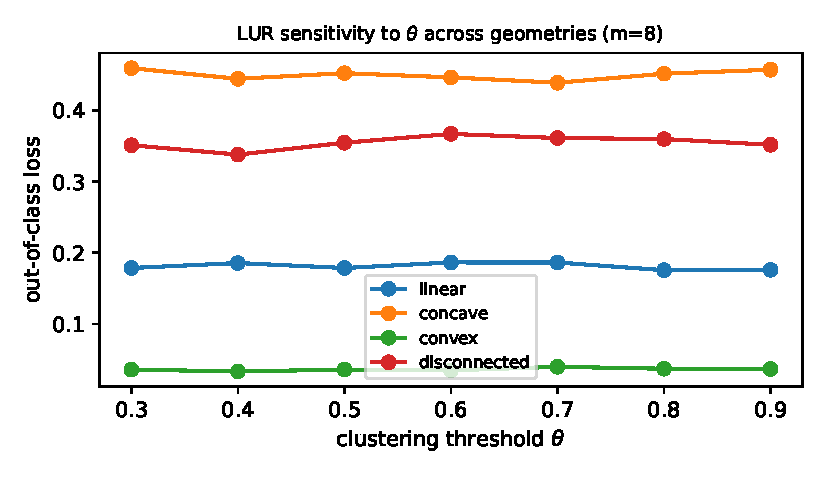
\includegraphics[width=\textwidth]{sensitivity_theta.pdf}\end{subfigure}
\hfill
\begin{subfigure}{0.48\textwidth}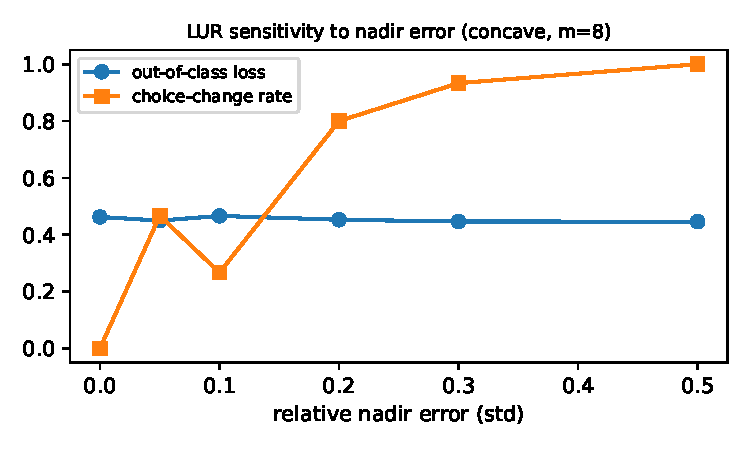
\includegraphics[width=\textwidth]{sensitivity_nadir.pdf}\end{subfigure}
\caption{Sensitivity of LUR. Left: held-out loss is flat in the clustering
threshold $\theta$ across all four geometries. Right: under nadir error the loss
stays stable while the recommendation changes more often (near-ties).}
\label{fig:sens}
\end{figure}

\subsection{Stochastic extension}
We validate the stochastic extension (Proposition~\ref{thm:stoch}) directly. On
noisy concave instances ($m=6$) we draw $n$ observations per criterion, form
plug-in means, and apply LUR; Figure~\ref{fig:stoch} reports how often the
resulting choice matches the noise-free LUR winner. Recovery rises monotonically
from $0.04$ at $n=1$ to $0.79$ at $n=100$, consistent with the consistency
statement (it does not reach $1$ because dense candidate sets contain near-ties,
exactly the situation the tolerance rule is designed for).

\begin{figure}[t]
\centering
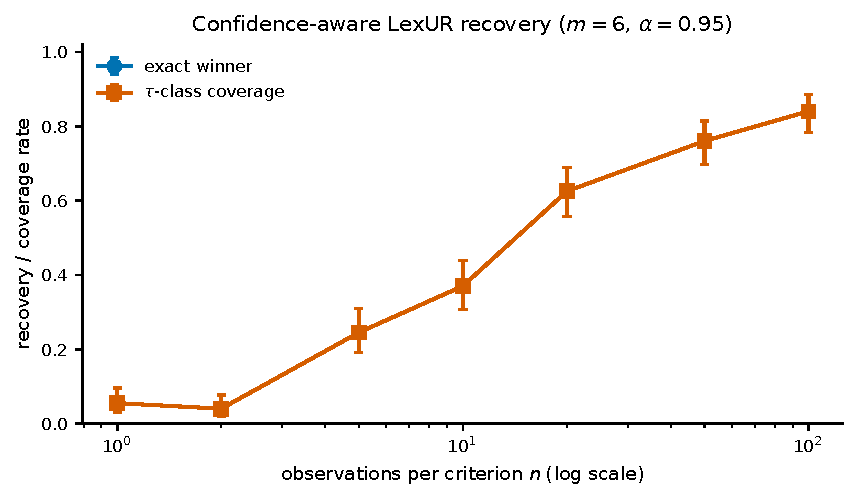
\includegraphics[width=0.6\textwidth]{stochastic_consistency.pdf}
\caption{Stochastic-LUR consistency: recovery rate of the noise-free winner vs.\
the number of observations per criterion (concave, $m=6$).}
\label{fig:stoch}
\end{figure}

\subsection{Pre-registered validation protocol and acceptance gates}
\label{sec:protocol}
To guard against confirmation bias we additionally ran a pre-registered protocol
(frozen config, single-command reproduction) on a deliberately broadened suite:
\textbf{eleven} methods (adding VIKOR, hypervolume contribution, and Chebyshev
minimax regret), \textbf{ten} held-out families spanning additive \emph{and}
non-additive preferences (adding sparse-linear, $L_p$, OWA, Choquet and
satisficing), Dirichlet weight shapes $\alpha\in\{0.2,1,5\}$, eight geometries and
$m$ up to $20$ ($2{,}400$ paired instances). The protocol fixes, in advance, a set
of \emph{acceptance gates}, each tied to one precise claim; we report the outcome
verbatim in Table~\ref{tab:gates} rather than only favourable numbers.

On this harder suite LUR has tail-loss rank $4.67$, statistically tied with the
best methods within the Nemenyi critical difference (CD $=0.31$): HV $4.27$,
ASF $4.65$, MMR $4.65$, LUR $4.67$, VIKOR $4.71$, ChebMMR $4.99$, then CP $5.32$,
TOPSIS $6.98$, knee $7.21$, RW $9.26$ and SMAA $9.30$ (Figure~\ref{fig:cdprot}).
A pre-registered \emph{non-inferiority} test (paired bootstrap, margin $0.01$
absolute \emph{or} $2\%$ relative) finds LUR non-inferior to both ASF and MMR
(upper 95\% CI bounds $0.004$ and $0.0025$), with negligible effect size
(Cliff's $\delta\le0.015$)---supporting ``practically equivalent to the best
robust scalarisations'' rather than ``better''. Direct computation is demonstrated
on a continuous linear MOP (LUR via sequential LPs uses $19$ solver calls and
\emph{no} front enumeration vs.\ $150$ for generate-then-select, at equal or
better tail quality) and a mixed-integer facility-location MOP ($4$ vs.\ $60$
solves for the same recommendation). The confidence-aware stochastic LUR attains
near-zero out-of-sample worst-criterion risk ($\approx0$) against $0.28$ for
TOPSIS and $0.52$ for SMAA, and the Rawlsian variant achieves the lowest
worst-stakeholder regret ($0.362$) and inequality (Gini $0.207$) among average-,
Nash- and max-min rules.

\begin{table}[t]
\centering\small
\caption{Pre-registered acceptance gates (reproduced at full scale). 9 PASS, 1 CHECK.}
\label{tab:gates}
\begin{tabular}{lll}
\toprule
Gate & Result & Evidence\\
\midrule
Dominated selections $=0$ & PASS & $0/150$ injections\\
Positive-affine invariance & PASS & $100\%$ identical\\
Nadir-error stability & CHECK & quality degr.\ $0.052$ (thr.\ $0.05$)\\
Non-inferior vs ASF (tail) & PASS & CI upper $0.004 < 2\%$ margin\\
Non-inferior vs MMR (tail) & PASS & CI upper $0.0025 < 0.01$ margin\\
Beats practical baselines (tail) & PASS & $\delta$: TOPSIS $.19$, CP $.06$, SMAA $.62$\\
Redundancy $<$ averaging (grouped) & PASS & $0.256$ vs $0.359$; cluster recovery $0.98$\\
Adaptive $\approx$ full (tail gap $\le0.01$) & PASS & gap $0.0096$\\
Direct computation (LP $+$ MILP) & PASS & $19$ vs $150$; $4$ vs $60$ solver calls\\
Stochastic LUR $\le$ deterministic (tail) & PASS & risk $\approx0$ vs $0.28/0.52$\\
\bottomrule
\end{tabular}
\end{table}

\begin{figure}[t]
\centering
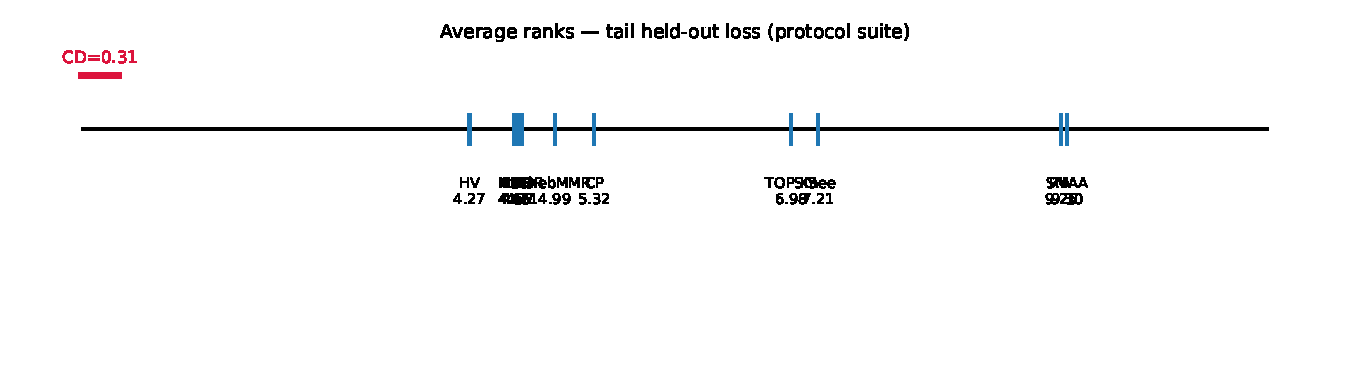
\includegraphics[width=0.92\textwidth]{cd_protocol.pdf}
\caption{Average ranks on tail held-out loss over the broadened protocol suite
(11 methods, 10 families, 8 geometries, $2{,}400$ instances; Nemenyi CD $=0.31$).
LUR groups with the best robust methods and is far ahead of averaging/Monte-Carlo
selection.}
\label{fig:cdprot}
\end{figure}

\subsection{Smart-grid dispatch case study}
We apply LUR to a six-objective stochastic 24-hour economic dispatch with ten
generators (cost, emissions, unreliability, ramping, non-renewable fraction, peak
gap) under Monte-Carlo renewable scenarios, yielding $163$ non-dominated dispatch
policies; the full dispatch model (demand profile, generator limits, ramping,
scenario generation) is specified in the released code.
Relative to the distance/averaging methods, LUR accepts a negligible increase in
\emph{mean} held-out loss ($0.103$ vs $0.100$) for a $23\%$ reduction in
\emph{worst-case} loss ($0.282$ vs $0.366$; knee $0.623$). Crucially it
\emph{explains} the choice: the certificate (Figure~\ref{fig:cert}) flags the
peak-shaving gap ($f_6$, regret $0.40$) and the non-renewable fraction ($f_5$,
$0.40$), then the ramping/peak coalition $\max(f_4,f_6)$ ($0.36$), telling the DM
not only which dispatch to adopt but where it remains fragile.

\begin{figure}[t]
\centering
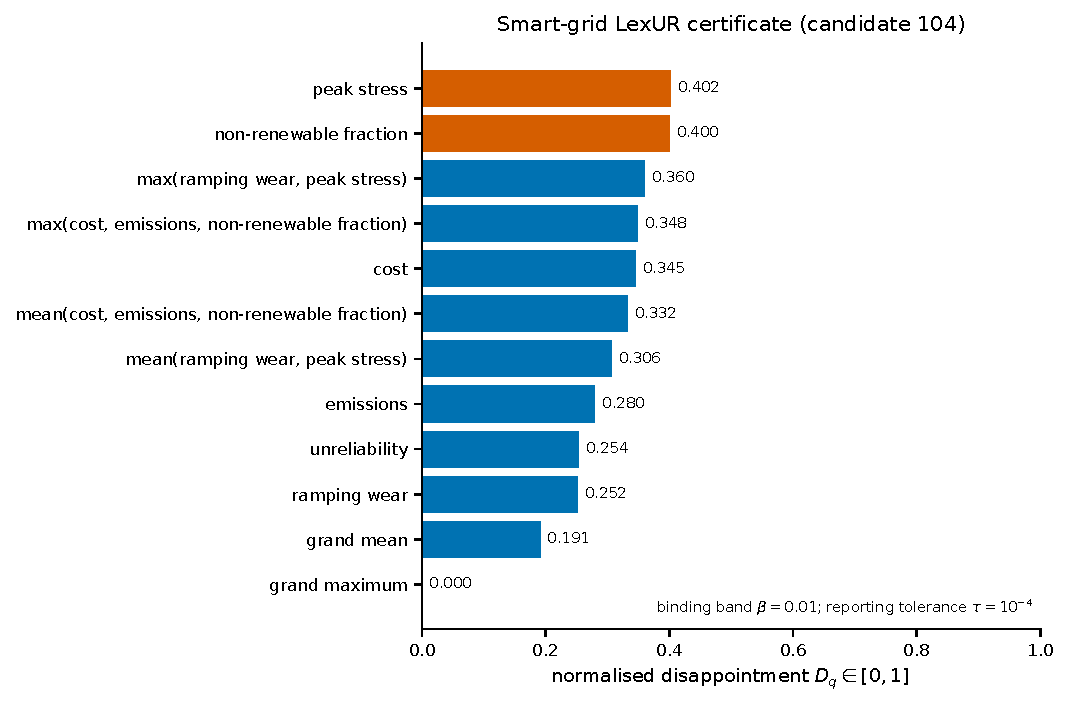
\includegraphics[width=0.7\textwidth]{certificate.pdf}
\caption{LUR regret certificate for the recommended smart-grid dispatch: the most
disappointed probes (peak gap $f_6$, non-renewable fraction $f_5$, and the
ramping/peak coalition) localise the fragility of the recommendation.}
\label{fig:cert}
\end{figure}
